\chapter{项目特色}

\section{Token 身份验证}
<<<<<<< HEAD
=======
Token身份校验是现代计算机系统中常用的一种安全措施,主要用于验证用户或设备的身份,确保系统的安全性。具体来说,token身份校验的作用包括:
用户身份验证,防止伪装攻击等。

\subsection{认证流程}
\begin{figure}[htbp]
	\centering
	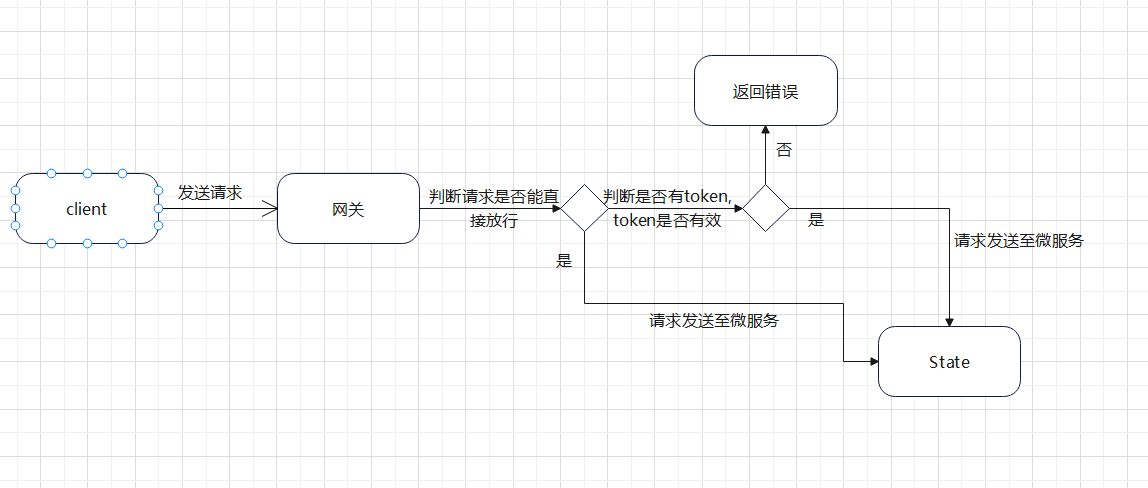
\includegraphics[width=1\textwidth,height=0.25\textheight]{token}
	\caption{token认证流程}\label{fig:token}
\end{figure} 

\subsection{Token分发}
主要在用户登录接口中实现了token分发,在用户成功登录之后,会将token存入redis缓存中,并将用户信息以及token返回给用户,实现如下:

\begin{lstlisting}[basicstyle=\footnotesize]
	@Override
	public LoginVo login(String username,String password) {
		User user = userMapper.getUserInfoByname(username);
		if (user == null){
			return null;
		}
		
		// 判断用户名密码是否正确
		if (!password.equals(user.getPassword())){
			return null;
		}
		// 生成token
		String token = jwtProvider.generateToken(user.getUserName());
		
		// 将token存入redis
		redisManager.set(UserConstant.USER_TOKEN_KEY_REDIS + user.getUserName(),token,604800);
		LoginVo lg = new LoginVo();
		lg.setToken(prefix + " " +token);
		lg.setUserId(user.getUserId());
		lg.setUserName(username);
		return lg;
	}
\end{lstlisting}

\subsection{Token认证}
token认证的功能主要实现在gateway的过滤器上。过滤器首先验证是否为放行路径,如果是直接将请求发送到微服务,如果不是会验证token是否存在,已经token是否有效,实现如下:
\begin{lstlisting}[basicstyle=\footnotesize]
	@Override
	public Mono<Void> filter(ServerWebExchange exchange, GatewayFilterChain chain) {
		
		ServerHttpRequest request = exchange.getRequest();
		String requestPath = request.getPath().toString();
		System.out.println(paths);
		System.out.println(requestPath);
		boolean allowedPath = false;
		if (paths != null && !paths.equals("")){
			allowedPath = requestPath.contains(paths);
		}
		if (allowedPath || StringUtils.isEmpty(requestPath)){
			return chain.filter(exchange);
		}
		
		// 验证token
		String authHeader = exchange.getRequest().getHeaders().getFirst(tokenHeader);
		if (authHeader != null && authHeader.startsWith(prefix)){
			String authToken = authHeader.substring(prefix.length());
			String userName = jwtProvider.getUserNameFromToken(authToken);
			
			// 查询redis
			Object token = redisManager.get(UserConstant.USER_TOKEN_KEY_REDIS + userName);
			if (token == null){
				
				return writeResponse(exchange.getResponse(),401,"token已过期...请重新登录");
			}
			
			String trimAuthToken = authToken.trim();
			if (! trimAuthToken.equals(token.toString())){
				return writeResponse(exchange.getResponse(),401,"token验证失败或已过期...请重新登录");
			}
		}else {
			return writeResponse(exchange.getResponse(),500,"token不存在");
		}
		return chain.filter(exchange);
	}
\end{lstlisting}
>>>>>>> 53eb9252 (完善报告结构)

\section{积分系统}
积分系统的设计参考了美团APP的米粒功能
\subsection{规则设计}
\subsubsection{积分获取}
\begin{enumerate}
	\item 签到获得积分,每日通过签到获得的积分上限为1次
	\item 消费时获得积分,订单金额按比例兑换为积分数量
	\item 充值时获得积分,将电子钱包的充值按比例转化为积分
\end{enumerate}
\subsubsection{积分消耗}
\begin{enumerate}
	\item 积分存在有效期,积分随着时间的增加自然减少
	\item 下单时可以通过消耗积分,来减少支付所需钱的数量
\end{enumerate}
\subsubsection{特殊的规则}
\begin{enumerate}
	\item 选择优先过期的积分进行消费
	\item 连续签到,节假日签到,特殊节日消费特殊商品等,有特殊的积分规则
\end{enumerate}

\subsection{数据库设计}

这里展示了积分规则的数据库图表,具体如下:

\begin{table}[htbp]
    \caption{积分记录表 (creditrecord)}
    \vspace{0.5em}\wuhao
    \begin{tabularx}{\hsize}{@{\extracolsep{\fill}}c c c}
    \toprule[1.5pt]
    字段名          	& 数据类型	 & 说明 \\ 
    \midrule[1pt]
    id      			& int      	& 主键id \\
    userId        		& varchar  	& 用户id \\
    ruleCode    		& varchar  	& 规则码 \\
    eventId 			& int  		& 订单/充值id \\
    credit 				& int  		& 积分值 \\
	createTime       	& datetime  & 创建时间 \\
    expiredTime       	& datetime  & 过期时间 \\
    \bottomrule[1.5pt]
    \end{tabularx}
\vspace{\baselineskip}
\end{table}

\begin{table}[htbp]
    \caption{可用积分表 (usablecredit)}
    \vspace{0.5em}\wuhao
    \begin{tabularx}{\hsize}{@{\extracolsep{\fill}}c c c}
    \toprule[1.5pt]
    字段名          & 数据类型  & 说明 \\ 
    \midrule[1pt]
    id      		& int      	& 主键id \\
    userId        	& varchar  	& 用户id \\
    recordId    	& int 		& 流水表记录id \\
    credit 			& int  		& 积分值 \\
    createTime 		& datetime  & 创建时间 \\
    expiredTime     & datetime  & 过期时间 \\
    deleted   		& int  		& 过期标记 \\
    \bottomrule[1.5pt]
    \end{tabularx}
\vspace{\baselineskip}
\end{table}

\begin{table}[htbp]
    \caption{积分扣除表 (reducecredit)}
    \vspace{0.5em}\wuhao
    \begin{tabularx}{\hsize}{@{\extracolsep{\fill}}c c c}
    \toprule[1.5pt]
    字段名          & 数据类型  & 说明 \\ 
    \midrule[1pt]
    id      		& int      	& 主键id \\
    userId        	& varchar 	& 用户id \\
    recordId    	& int  		& 流水表中消费积分记录id \\
    usableId 		& int  		& 可用积分表中对应的记录id \\
    credit 			& int  		& 积分值 \\
	createTime      & datetime  & 创建时间 \\
    expiredTime     & datetime  & 过期时间 \\
    \bottomrule[1.5pt]
    \end{tabularx}
\vspace{\baselineskip}
\end{table}

\begin{table}[htbp]
    \caption{积分规则表 (creditrule)}
    \vspace{0.5em}\wuhao
    \begin{tabularx}{\hsize}{@{\extracolsep{\fill}}c c c}
    \toprule[1.5pt]
    字段名          & 数据类型  & 说明 \\ 
    \midrule[1pt]
    id      	& int      	& 主键id \\
    ruleCode    & varchar  	& 积分规则码 \\
	type      	& int      	& 获取/消费 \\
	priority    & int      	& 优先级 \\
	credit 		& int  		& 积分值 \\
	formula 	& int 		& 公式 \\
	dalyCap 	& int 		& 日上限 \\
	totCap 		& int 		& 总上限 \\
	startTime   & datetime  & 开始时间 \\
    endTime     & datetime  & 结束时间 \\
	lifespan 	& int 		& 有限期 \\
	state 		& int 		& 启用/停用 \\
    \bottomrule[1.5pt]
    \end{tabularx}
\vspace{\baselineskip}
\end{table}



\subsection{接口设计}

\textbf{查询当前可用积分}

CreditController/queryAvailableCredit

参数:userId

返回值:int

功能:查找userId用户的所有可用积分

\textbf{查询积分流水}

CreditController/queryAllCredit

参数:userId

返回值:List(记录积分的数组)

功能:查找userId用户的所有专区或者消费的积分明细

\textbf{签到获得积分}

CreditController/earnCreditBySign

参数:userId,creditNum,ruleCode

返回值:int

功能:签到获得积分,每日通过签到获得的积分上限为1次

\textbf{查询签到可以获得的积分总数}

CreditController/queryEarningCreditBySign

参数:userId,ruleCode

返回值:int

功能:查找userId用户,在规则码为ruleCode的情况下,能够获取的积分总数

\textbf{查询支付可以获得的积分总数}

CreditController/queryEaringCreditByPaying

参数:userId,money,ruleCode

返回值:int

功能:给所有userId的用户查询支付money的钱可以获得多少积分

\textbf{支付后获得积分}

CreditController/earnCreditByPaying

参数:userId,orderId,creditNum,ruleCode

返回值:int

功能:让用户支付之后获得积分

\textbf{支付时抵扣积分}

CreditController/queryConsumingCreditByPaying

参数:userId,money,creditNum,ruleCode

返回值:creditNum,deductionMoney

功能:让用户在支付时使用积分做抵扣

\section{虚拟钱包系统}
参考美团APP的天天神券功能,制作了一个虚拟支付钱包。

\subsection{规则设计}
\subsubsection{电子钱包的创建}
\begin{enumerate}
	\item 用户同意时,主动创建一个钱包
	\item 商家需要主动与平台完成签约创建钱包
\end{enumerate}

\subsubsection{支付逻辑}
\begin{enumerate}
	\item 优先消耗积分支付
	\item 必须保证钱包扣款的线程安全
	\item 保障支付本身的事务性
\end{enumerate}

\subsection{具体实现}
在定义上,我们不仅采用了~pojo~层,还采用了~VO~层,其中,~pojo~层又叫~PO~,是面向数据库的,与其协同的对象分别为~Service~层和~Dao~层,放从数据库中直接拿出来的数据,没有任何逻辑实现,只有~getter~域~setter~方法,数据库的每一个字段都对应着~POJO~的一个属性。
~VO~是面向~Service~层与~Controller(Web)~层的,~VO~的数据是~POJO~中的数据加工后得到的,用于在~Web~页面上展示。

\begin{lstlisting}[basicstyle=\footnotesize]
package com.tju.elmcloud.po;

public class VirtualWalletPo {
	private String userId;
	private Integer walletId;
	private double balance;

	public VirtualWalletPo(){
		this.balance=0.00;
	}
	public VirtualWalletPo(Integer walletId,double balance){
		this.balance=balance;
		this.walletId=walletId;
	}
	public Integer getWalletId() {
		return walletId;
	}
	public double getBalance() {
		return balance;
	}
	public String getUserId() {
		return userId;
	}
	public void setUserId(String userId) {
		this.userId = userId;
	}
}	
\end{lstlisting}
		
\subsection{保障事务性}
在本项目中,为了保证钱包支付的事务性,我们采取了~synchronized~和自带线程安全的~cocurrentHashMap~来实现,具体为在操作线程钱进行加锁,来保证关于金钱操作的~ACID~事务性。
这里以~queryEarningCreditBySign~方法举例。

\begin{lstlisting}[basicstyle=\footnotesize]
@Override
public Integer queryEarningCreditBySign(String userId) {
	Integer ruleId = 1;
	String time = CommonUtil.getCurrentDate();
	String today = time.substring(0, time.indexOf(' ')).trim();
	int count = creditRecordMapper.todaySignRecord(userId, ruleId, today);
	SignCreditRule signCreditRule = null;
	synchronized (creditRuleMap) {
		signCreditRule = (SignCreditRule) creditRuleMap.getRule(ruleId);
		if (signCreditRule == null) {
			CreditRulePo creditRulePo = creditRuleMapper.getRule(ruleId);
			int credit = creditRulePo.getCredit();
			int lifeSpan = creditRulePo.getLifespan();
			int totCap = creditRulePo.getDailyCap();
			signCreditRule = new SignCreditRule(lifeSpan, credit, totCap);
			creditRuleMap.writeMap(ruleId, signCreditRule);
		}
	}
	CreditSystem creditSystem = new CreditSystemImpl();
	return creditSystem.queryEarningCreditBySign(count, signCreditRule);
}
\end{lstlisting}

